\documentclass[tikz]{standalone}

\usepackage{amsmath}
\usepackage{mathrsfs}
\usetikzlibrary{positioning}

\usepackage{amsmath}
\usepackage{mathrsfs}

\newcommand{\cat}[1]{\mathscr{#1}}
\newcommand{\obj}[1]{|#1|}
\newcommand{\mrp}[3]{#1(#2,#3)}
\newcommand{\id}[1]{\mathrm{id}_{#1}}
\DeclareMathOperator{\dom}{dom}
\DeclareMathOperator{\cod}{cod}
\DeclareMathOperator{\colim}{Colim}
\DeclareMathOperator{\lan}{Lan}
\DeclareMathOperator{\ran}{Ran}


\begin{document}
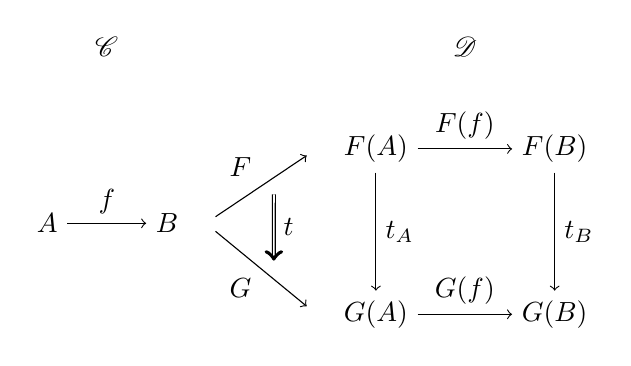
\begin{tikzpicture}
	\node (catc) {$\cat{C}$};
	\node [below left=2cm and 0.5cm of catc.center] (A) {$A$};
	\node [right=1.0cm of A] (B) {$B$};
	\node [right=4.0cm of catc] (catd) {$\cat{D}$};
	\node [below left=1cm and 0.6cm of catd.center] (FA) {$F(A)$};
	\node [right=1.2cm of FA] (FB) {$F(B)$};
	\node [below=1.8cm of FA.center] (GA) {$G(A)$};
	\node [below=1.8cm of FB.center] (GB) {$G(B)$};
	\draw [->] (A) to node [above] {$f$} (B);
	\draw [->] (FA) to node [above] {$F(f)$} (FB);
	\draw [->] (GA) to node [above] {$G(f)$} (GB);
	\draw [->] (FA) to node [right] {$t_A$} (GA);
	\draw [->] (FB) to node [right] {$t_B$} (GB);
	\node [right=0.1cm of B] (from) {};
	\node [left=0.1cm of FA] (fto) {};
	\draw [->] (from) to node [above left] (F) {$F$} (fto);
	\node [left=0.1cm of GA] (gto) {};
	\draw [->] (from) to node [below left] (G) {$G$} (gto);
	\node [below right=0.1cm and 0.3cm of F.center] (tfrom) {};
	\node [above right=0.1cm and 0.3cm of G.center] (tto) {};
	\draw [->,double] (tfrom) to node [right] {$t$} (tto);
\end{tikzpicture}
\end{document}
